% !TeX spellcheck = en_GB
% This is LLNCS.DOC the documentation file of
% the LaTeX2e class from Springer-Verlag
% for Lecture Notes in Computer Science, version 2.4
\documentclass{llncs}
\usepackage{llncsdoc}
\usepackage{graphicx} 
\usepackage{booktabs}
\usepackage{amsmath}
\usepackage{amssymb}
\usepackage{amsmath}
\usepackage{mathtools}

\usepackage[linesnumbered,ruled]{algorithm2e}

\usepackage[noend]{algpseudocode}

\newcommand{\R}{\mathbb{R}}
%
\begin{document}
\thispagestyle{empty}
\rule{\textwidth}{1pt}
\vspace{2pt}
\begin{flushright}
\Huge
\begin{tabular}{@{}l}
Barriers to the\\
implementation of\\
k-anonymity and\\
related microdata\\
anonymization techniques\\
in a realworld application\\[6pt]

\end{tabular}
\end{flushright}
\rule{\textwidth}{1pt}
\vfill
\title{Barriers to the implementation of k-anonymity and related microdata anonymization techniques in a realworld application}
\author{Andreas Wiegnand, 1878334\\
	Ludwig Schallner, 1850413}
\institute{}
\maketitle
%
%\tableofcontents
\section*{Abstract}
\textit{At first sight, implementation of k-anonymity appears to be an easy task for the developer. However, previous studies have concentrated separately on the barriers of implementation. This paper aims to present a completed overview of the barriers, which play the most important role and have the highest impact on k-anonymity. By means of examples it will be supported that data distortion is a barrier, since the more generalised the data are, the more information the researcher will have to sacrifice. Attacks, such as the Homogeneity, Background Knowledge and the Unsorted Matching Attack, will also be considered as barriers. In addition, this paper discusses NP-Hardness as a barrier. Furthermore, algorithms such as the KACA, OLA and the Cloaking algorithm, which address some of these barriers, will be addressed at the end of this paper.}
\newpage
\setcounter{page}{1}

\section{Introduction}
%
Nowadays data are a key factor in almost every domain. It is comparable to the gold rush of the $19^{th}$ century \cite{datarevo}. Furthermore, storage space and network ability become increasingly affordable \cite{sweeney2002k}. 
This is leading to an open-source community where the created and stored data are not only useful to the original data holder, but also to other researchers. In some cases the data are only useful when they are combined and analysed together with other data. However, those data may contain some personal or sensitive information; thus the data should only get released if their privacy is secured  \cite{li2006achieving}.\\
\begin{table}[]
	\centering
	\caption{Basic example}
	\label{intro_example}
	\begin{tabular}{@{}llll@{}}
		\toprule
		SSN         & Age & Postcode & Problem         \\ \midrule
		680-90-2665 & 25  & 4568     & procrastination \\
		008-07-4179 & 34  & 4567     & stress          \\
		391-05-7998 & 48  & 4569     & stomach cancer  \\
		078-36-3853 & 39  & 4568     & obesity         \\
		411-71-9290 & 42  & 4561     & stomach ulcers  \\
		527-59-1948 & 27  & 4568     & stress          \\ \bottomrule
	\end{tabular}
\end{table}

The data presented \textit{Table \ref{intro_example}} must first be anonymized before their release is approved. A very common technique to achieve this goal is the so-called k-anonymity process, which prevents the danger of private data leakage. This paper aims to show the barriers to the implementation of k-anonymity. Section 1 will present the required theoretical background to understand k-anonymity and its purpose. Section 2 will discuss the underlying barriers of k-anonymity, while Section 3 takes into consideration the possible attacks of k-anonymity, which might function as barriers to this process. Section 4 explains how multiple algorithms can be implemented k-anonymity. A summary of the implementations of this process and its possible barriers  will be provided in the last section of this paper.
\newpage
\section{Basics}
In order to understand the process of k-anonymity one should be familiar with its basic concepts. This is possible by presenting and explaining in detail the theoretical background.  The first term to be introduced is \textit{microdata}. The data being processed contain records of information about individuals.Microdata is more aggregate than usual data and it is also naturally accessible, since everyone who has these data can run his/her own statistics from it \cite{microdataweb}. 
Another important term is \textit{Identifier}. These are attributes which can detect explicitly the record owner without any other attribute. For example, the owner’s full name (first and last name), telephone number, social security number, and even more specific private data \cite{domingo2008critique}.\\\\
In order to anonymize the data, \textit{identifier} is removed from the published data. However, there is another process that are retained are the so-called \textit{Quasi-identifier}. These are attributes which non-explicitly identify the record owner. When they are combined with other non-explicit attributes or other tables, they can re-identify the record owner. In such cases these combinations of attributes are called quasi-identifier, such as \textit{gender}, \textit{age}, \textit{postcode}, \textit{weight} and \textit{height} \cite{dalenius1986finding}. An example of this process is to be found in figure \ref{quasiidentifier} (the quasi-identifier of figure would be ZIP (postal code), birth date and sex).\\
\begin{figure}[]
	\centering
	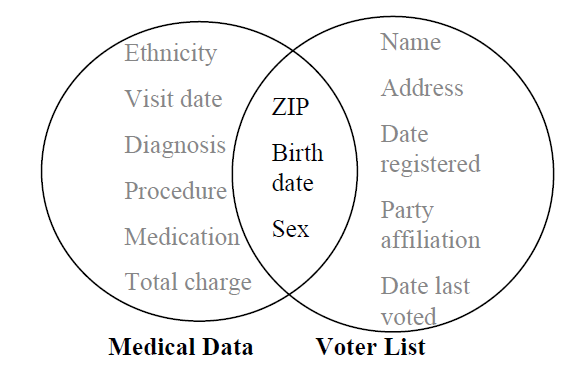
\includegraphics[width=0.6\textwidth]{linkingdata.png}
	\caption{Quasi-identifiers \cite{sweeney2002k}}%
	\label{quasiidentifier}
\end{figure}\\
The most important type of data worth mentioning is \textit{sensitive data}. This type of data is useful to researchers but they contain private information and should not be publicized or be accessible to strangers. Record owners do not want to be linked to these type of data. Next to data types there are 3 ground knowledge types: \textit{Background knowledge}, \textit{Instance-level background knowledge}, and \textit{Demographic background knowledge}. \textit{Background knowledge} deals with the uncertainty of the amount of data access the attackers has. The developer has to consider that the attackers might have access to a table, and they might know that in order to achieve k-anonymity tables are generalized. Furthermore, the attackers are aware of the domain attributes. Instance-level background knowledge, then, reveals that the adversary possesses comprehensive knowledge of the target’s specific details. For example, Alice (the adversary) knows that Bob does not suffer from a disease, because he has no symptoms. In this case, Alice can conclude of what actually Bob suffers from. Lastly, in the demographic background knowledge the adversary is informed about general facts, for example P (t[condition] = cancer| t[Age] $\geq$ 40). With these information the attackers can access and interference the records \cite{ldiversity}.\\\\
Considering \textit{K-Anonymity}, the main goal of making a k-anonymized table is to have at least (k-1) tuples of each identical tuple by taking the corresponding quasi-identifiers into account  \cite{sweeney2002k,li2006achieving}. For example, the k-anonymized version of \textit{Table  \ref{intro_example}} in the introduction section would be the following table:
\begin{table}[]
	\centering
	\caption{Basic example 2-anonymized}
	\label{intro_example_sol}
	\begin{tabular}{@{}llll@{}}
		\toprule
		SSN         & Age & Postcode & Problem         \\ \midrule
		* & 2*  & 456*     & stress \\
		* & 3*  & 456*     & stress          \\
		* & 4*  & 456*     & stomach cancer  \\
		* & 3*  & 456*     & obesity         \\
		* & 4*  & 456*     & stomach ulcers  \\
		* & 2*  & 456*     & stress          \\ \bottomrule
	\end{tabular}
\end{table}\\
The set of all tuples with the identical quasi-identifiers of a table are referred as equivalence class \cite{li2006achieving}.\\\\
%%%%%%
It is also important to note that there are two kinds of disclosure. On the one hand there is \textit{ identity disclosure}, during which an individual identity is detected and matched to a particular record. On the other hand there is \textit{attribute disclosure}, during which new information are linked to an individual. For example, Bob is linked to his record in \textit{Table \ref{intro_example_sol}}, because of an attack (see Section 3.3). The adversary discovers that he suffers from stress \cite{sweeney2002k}.\\\\
The last two terms concerning the basic concepts of k-anonymity are \textit{global recoding/domain generalisation} and \textit{local recording}. The first refers to a very common generalization technique during which once an attribute value is generalized then all occurrences of that value are replaced by the generalized one  \cite{sweeney2002k,sweeney2002achieving,li2006achieving,incognito}. The later entails coding strategies, which work differently from the ones described above. \textit{Local recording} generalizes the attribute values in cells. Consequently, these types of strategies do not over generalize the table and the data distortion is significantly lower \cite{li2006achieving}. 
 
\section{Underlying Barriers}

In the following section, the paper will present the basic and most challenging barriers to the implementation of k-anonymity. The barriers, which can emerge during the implementation of k-anonymity, will be explained further. These are the so-called \textit{distortion of data}, or as mentioned in some papers \textit{data loss} or \textit{information loss}, attacks on k-anonymity and the NP-Hardness. 
\subsection{Distortion of data as Barrier} \label{sec:Distortion of data as Barrier}

A basic underlying barrier of k-anonymity is the process of measuring whether an implementation has been successful or whether it leads to a satisfying result. This can be measured by a simple calculation. The \textit{modification rate} denotes the fraction of cells which are modified within the attribute set of the quasi-identifier \cite{li2006achieving}.

	
\begin{table}[]
	\centering
	\caption{a: original table, b: example for local recording, c: example for domain generalization }
	\label{table_distortion}
	\begin{tabular}{@{}lllllllllll@{}}
		\multicolumn{3}{c}{\textbf{a}} &           & \multicolumn{3}{c}{\textbf{b}} &  & \multicolumn{3}{c}{\textbf{c}} \\ \midrule
		Gender  & Birthday   & Problem & \textbf{} & Gender  & Birthday   & Problem &  & Gender  & Birthday  & Problem  \\ \midrule
		male    & 13.08.1962 & stress  &           & male    & 13.08.1962 & stress  &  & *       & 196*      & stress   \\
		male    & 28.10.1967 & obesity &           & male    & 28.10.1967 & obesity &  & *       & 196*      & obesity  \\
		male    & 20.01.1977 & stress  &           & *       & 197*       & stress  &  & *       & 197*      & stress   \\
		female  & 15.09.1973 & obesity &           & *       & 197*       & obesity &  & *       & 197*      & obesity  \\
		female  & 15.03.1985 & stress  &           & female  & 15.03.1985 & stress  &  & *       & 198*      & stress   \\
		female  & 28.05.1986 & obesity &           & female  & 28.05.1986 & obesity &  & *       & 198*      & obesity  \\ \bottomrule
	\end{tabular}
\end{table}

As can be observed in \textit{Table \ref{table_distortion}b}, the modification rate is  33,$\overline{33}$\% (4 out of 12 quasi-identifier are changed) but for \textit{Table \ref{table_distortion}c} the rate is 100\% (12 out of 12 quasi-identifier got changed). As it can be seen in this simple example, the modification rate calculation is an unsatisfying procedure. Due to this, Li, Wong, Fu and Pei introduced the \textbf{weighted hierarchical distance}. In order to calculate the weighted hierarchical distance of a cell which is generalized from level p to level q, the following formula is used\\
%%%%%%%%%%%%%%%%%%
%%%FORMEL%%%%%%%%%
%%%%%%%%%%%%%%%%%%
\scalebox{1.25}{$ WHD (p, q) = \frac{\sum_{j=q+1}^{p} \omega_{j,j-1}}{\sum_{j=2}^{h} \omega_{j,j-1}} $}\cite{li2006achieving}.\\
%%%%%%%%%%%%%%%%%%
%%%FORMEL%%%%%%%%%
%%%%%%%%%%%%%%%%%%
Let the hierarchy of birth date be \{D/M/Y, M/Y, Y, 10Y, C/T/G/P, *\}. Where D/M/Y  stands for day.month.year, 10Y a 10 years interval and C/T/G/R for Child/Teen/Grownup/Pensioner.
\\\\
Another example can be shown by having a uniformed weight $w_{j,j-1} = 1$ where $2\leq j \leq h$ \cite{li2006achieving}. By using the aforementioned example Birthday is generalized from D/M/Y to 10Y, which corresponds into $WHD_{Birthday}(6,3) = \frac{3}{5} = 0,6$. 
The Gender generalization would be $WHD_{gender}(2,1) = \frac{1}{1} = 1$. In such, in order to generalize 5 cells of age from D/M/Y to 10Y, one has to do the same data distortion as when 3 cells of gender are generalized from Male/Female to *. This calculation presents a much better way to address the distortion of data than the modification rate. However, this does not take into account how close is the generalization to the root (which would be *).\\\\
A last example can be shown with height weight $w_{j,j-1} = 1 / (j-1)^{\beta}$ where 2 $\leq$ j $\leq$ h and $\beta = \R \geq$ 1 \cite{li2006achieving}:
$\beta$ can be chosen by the user. For example $\beta = 1$. For $WHD_{Birthday}(6,3) = \frac{0,\overline{33}+0,25+0,20}{1+0.5+0,\overline{33}+0,25+0,20} \sim 0,3431$. For $WHD_{gender}(2,1) = \frac{1}{1} = 1$. The distortion of 3 changed cells of birthday, i.e. from D/M/Y to 10Y, has the same impact on the distortion of data as when only one cell, i.e. from Female/Male to *, gets generalized.\\\\
Coming to a conclusion the researcher demands the information provided in the tables, as shown in these examples. Therefore, it is very important that the least possible information are lost during the anonymization process. In order to understand the importance of this aspect, consider another example. You have a table with survivors from a disaster beyond all expectations. Researchers will try to discover the long-term effects of this disasters and whether the victims are more likely to live a long and happy life by measuring their distance from disaster’s location. If there is a mass generalization of by the location (ZIP), it might be useless or non-significant for researchers to work with this information.
%%%%%%
%% DONE %%%
%%%%%%%%%%%%%
\subsection{Attacks as Barrier}

Attacks can be considered as another barrier to k-anonymization implementations. If the implementation ignores the deficiencies which the attacks can make use of, k-anonymity has then no value. It is absolutely necessary that an attacker, under no circumstances, discovers information about the target while he/she is reading the published database. This should also be feasible even if the attacker has background knowledge of other sources   \cite{Dalenius1977}. Unfortunately, as shown by Dwork such safety parameters are impossible, because of the unfeasibility to predict what the attacker might know \cite{dwork2011differential}. Therefore, it is important and necessary that the implementation takes possible attacks into account and implements countermeasures. However, since attacks are not the main focus of this paper, a rather short introduction will be provided.\\\\
One type of an attack is the so-called \textit{Homogeneity Attack}. Let Alice be the adversary and let be Bob her target. They are neighbours and one day Bob is transported with an ambulance to the hospital. Let us assume that the hospital published the \textit{Table \ref{homogenityattack}}, where all current patients including their \textit{Nationality, Age, ZIP,} and \textit{Problem}, are listed, is already k-anonymized before its release. Alice knows that Bob is a 31 years old, American who lives in 02239 (ZIP Code). Thus, she can conclude that he is entry 3, 5,6, or 11.\\\\
Furthermore, all of these entries have the same Problem: Cancer. Alice can conclude that Bob suffers from cancer even if the table the table has already been k- anonymized  \cite{sweeney2002k,ldiversity}. To counteract such attacks diversity is needed. One method which is worth mentioning, but will not be further discussed in this paper is the so-called l-diversity \cite{ldiversity}.  

% Please add the following required packages to your document preamble:
% \usepackage{booktabs}
\begin{table}[]
	\centering
	\caption{Homogeneity attack}
	\label{homogenityattack}
	\begin{tabular}{@{}llllllllll@{}}
		\cmidrule(lr){2-5} \cmidrule(l){7-10}
		& Nationality     & Age & ZIP   & Problem         &  & Nationality & Age      & ZIP   & Problem         \\ \cmidrule(lr){2-5} \cmidrule(l){7-10} 
		1  & American        & 42  & 02135 & Viral Infect    &  & *           & $\geq$40 & 021** & Viral Infect    \\
		2  & Japanese        & 41  & 02133 & Hearth disease  &  & *           & $\geq$40 & 021** & Hearth disease  \\
		3  & Germany         & 38  & 02238 & Hearth disease  &  & *           & 3*       & 0223* & Cancer          \\
		4  & Japanese        & 29  & 02139 & Fever           &  & *           & $\leq$30 & 021** & Fever           \\
		5  & Indina          & 37  & 02232 & Viral Infection &  & *           & 3*       & 0223* & Cancer          \\
		6  & Native-american & 34  & 02236 & Cancer          &  & *           & 3*       & 0223* & Cancer          \\
		7  & Russia          & 53  & 02138 & Viral Infection &  & *           & $\geq$40 & 021** & Viral Infection \\
		8  & China           & 23  & 02139 & Cancer          &  & *           & $\leq$30 & 021** & Cancer          \\
		9  & American        & 23  & 02141 & Short of breath &  & *           & $\leq$30 & 021** & Short of breath \\
		10 & Indian          & 46  & 02139 & Viral Infection &  & *           & $\geq$40 & 021** & Viral Infection \\
		11 & American        & 31  & 02239 & Vomiting        &  & *           & 3*       & 0223* & Cancer          \\
		12 & American        & 28  & 02130 & Viral Infection &  & *           & $\leq$30 & 021** & Viral Infection \\ \cmidrule(lr){2-5} \cmidrule(l){7-10} 
	\end{tabular}
\end{table}

Another type of an attack is the \textit{Background Knowledge Attack}. This type of an attack uses demographic background knowledge, which is stored in the ground information of an adversary. Let us assume that Alice has a colleague, who enters also to the same hospital. This colleague is a 32 years old, Japanese and lives in 93607 (ZIP). Everyone with the same quasi-identifiers, i.e. Age = 3* and ZIP = 936**) have cancer or a heart disease. However, she knows that Japanese have a very low risk of a heart disease and, thus, she concludes that her college has cancer \cite{ldiversity}.
\begin{table}[]
	\centering
	\caption{Background Knowledge Attack}
	\label{tablebackground}
	\begin{tabular}{@{}llllllll@{}}
		\cmidrule(r){1-4} \cmidrule(l){6-8}
		& ZIP Code & Age & Disease        &  & ZIP Code & Age      & Disease        \\ \cmidrule(r){1-4} \cmidrule(l){6-8} 
		1 & 93677    & 29  & Liver Disease   &  & 936**    & $\leq$30 & Liver Disease   \\
		2 & 93602    & 22  & Liver Disease   &  & 936**    & $\leq$30 & Liver Disease   \\
		3 & 93909    & 52  & Cancer         &  & 9390*    & $\geq$40 & Cancer         \\
		4 & 93906    & 47  & Flu            &  & 9390*    & $\geq$40 & Flu            \\
		5 & 93673    & 36  & Hearth Disease &  & 936**    & 3*       & Hearth Disease \\
		6 & 93607    & 32  & Cancer         &  & 936**    & 3*       & Cancer         \\ \cmidrule(r){1-4} \cmidrule(l){6-8} 
	\end{tabular}
\end{table}

The last type of attack that will be shown in this table is the \textit{Unsorted Matching Attack} against k-anonymity. This type of attack is based on the very common strategy to release two tables separately. For example, let us assume a two column weight \textit{Table \ref{MatchingAttack}a}. This table can then be separated into two tables (6b, 6c). \textit{Table \ref{MatchingAttack}b} will contain \textit{Age} completely generalized but ZIP ungeneralized, and \textit{Table \ref{MatchingAttack}c} will have \textit{Age} ungeneralized but ZIP is generalized. The adversary can simply merge both tables and obtain \textit{Table \ref{MatchingAttack}a}, and have access to sensitive information. This weakness can be solved through random sorting \cite{meyerson2004complexity}.

\begin{table}[]
	\centering
	\caption{Unsorted Matching Attack example}
	\label{MatchingAttack}
	\begin{tabular}{@{}cccccccc@{}}
		\multicolumn{2}{c}{\textbf{a}} & \multicolumn{1}{l}{} & \multicolumn{2}{c}{\textbf{b}} & \multicolumn{1}{l}{} & \multicolumn{2}{c}{\textbf{c}} \\ \cline{1-2} \cline{4-5} \cline{7-8} 
		Age           & ZIP            &                      & Age           & ZIP            &                      & Age           & ZIP            \\ \cline{1-2} \cline{4-5} \cline{7-8} 
		42            & 91058          &                      & *             & 91058          &                      & 42            & 91050          \\
		44            & 91058          &                      & *             & 91058          &                      & 44            & 91050          \\
		50            & 27785          &                      & *             & 27785          &                      & 50            & 27780          \\
		52            & 27785          &                      & *             & 27785          &                      & 52            & 27780          \\
		20            & 32105          &                      & *             & 32105          &                      & 20            & 32100          \\
		21            & 32105          &                      & *             & 32105          &                      & 21            & 32100          \\
		31            & 67676          &                      & *             & 67676          &                      & 31            & 67670          \\
		32            & 67676          &                      & *             & 67676          &                      & 32            & 67670          \\ \cline{1-2} \cline{4-5} \cline{7-8} 
	\end{tabular}
\end{table}

Drawing a conclusion from the possible attacks on \textit{k-anonymity}, it should be clear that before the implementation of \textit{k-anonymity} the application has to be tested for such attacks it should also be secured against any other possible attacks.

\subsection{NP-Hard}
Meyerson and Williams analyzed the complex production of an optimal K-anonymity solution and discovered there is an NP-Hard Problem. Which means that the problem is at least NP-Complete but maybe harder. This might suggest that the Algorithm which should produce an optimal K-anonymity will not find a possible solution. Concerning a real world application, this means that the production of a k-anonymity solution with the least possible information loss is not feasible. However they show an approximation algorithm for k-anonymizing, which will take polynomial time and will use suppression the most O(k log k)  \cite{sweeney2002k}. The problem with suppression is the high information loss it produces. So someone had to choose between time complexity and information loss as a barrier for the implemenation of k-anonymity \cite{el2009globally}. 



\section{Algorithm}
This section will show some algorithms which goals is to archive \textit{k-anonymity} through generalization. These algorithms are also examples for barriers of k-anonymity implementation. 

\subsection{The KACA Algorithm}{Kaca}
The idea behind this algorithm idea is to achieve \textit{k-anonymity} by clustering attribute hierarchical structures. The algorithm chooses a random \textit{equivalent class}, which is smaller than k. The next step is to form a lager \textit{equivalent class} by merging the chosen one with the closest \textit{equivalent class}. This is resulting in a larger combined \textit{equivalent class}. Through repeating this process the end result is that each \textit{equivalent class} consists of at least k-tuples \cite{li2006achieving}.\\
\begin{algorithm}[H]
	\caption{K-Anonymization by Clustering in Attribute hierarchies (KACA) \cite{li2006achieving}}
	form equivalence classes from the data set\\
	\While{there exists an equivalence class of size $<$ k}{
	randomly choose an equivalence class $C$ of size $k$ k\\
	evaluate the pairwise distance of $C$ and all other equivalence classes\\
	find the equivalence class $C'$ with the smallest distance to $C$\\
	generalise the equivalence classes $C$ and $C'$
	}	
\end{algorithm}
This algorithm has a runtime of $O(nlogn + |E|^{2})$. Li, Wong, Fu, and Pei have shown that their \textit{KACA-Algorithm} is resulting in a 5.57 times smaller amount of distortion as the well known \textit{Incognito Algorithm}. The reason is lying in the technique which \textit{Incognito} is using. Its a global recoding algorithm, which is resulting in a over-generalized table \cite{li2006achieving}. Therefore, for less information loss, which is important for researchers an algorithm like KACA should be used.


\subsection{The Optimal Lattice Anonymization(OLA) Algorithm}

The OLA Algortihm was original produced for the field of health data anonymization. The goal of OLA is  to prodcue optimal k-anonymity. That means producing the usual definition of k-anonymity with the differents to produce less information loss as possible. In chapter \ref{sec:Distortion of data as Barrier} was shown one possibilty of measuring the information loss. 
The Algortihm can use three different kind of information loss metrices which result in different anonymization result. Information loss can result in loss of statistical power, inaccurate analysis result and inefficient use of data.  The alogrithem works with supression and generalization of the data. Supression can result in drastical information loss due to the fact that a hole attribute gets removed.\\

\begin{figure}
	\centering
	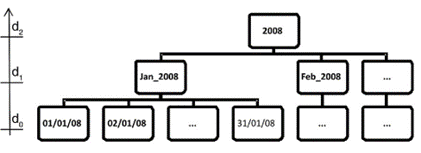
\includegraphics[width=0.6\textwidth]{general1.png}
	\caption{Generalization\cite{el2009globally}}%
	\label{Generalization}
\end{figure}



Generalization will be performed on all potential quasi identifiers. An example for generalization can be found in figure \ref{Generalization}. For different kind of data there a different kind of genralization technics. Thus, for strings the rightmost char can be deleted, while for numerical data the developer can produce intervals which will include the generalized attribute. Concerning dates, the developer can reduce the specification from days to months up to years. Generalization includes supression. The highest attribute on each generalization lattice is the suppressed version of the attribute and it also excludes every information\cite{el2009globally}. 

The most time consuming operation is to first find all the K-anonymous solutions in a dataset and then to compare them to each other with respect to their information loss. In order to achieve better performance at step1, the OLA algorithm uses Predictive Tagging, which enhances the process. The process of tagging takes advantage of the structure of the generalization lattice. A lattice is found in Figure \ref{lattice}. In its turn, every note in the generalization lattice is tested about it´s k-anonymity. If a k-anonymous node was found on hight n. All notes above n and in the same generalization strategy are also k-anonymous. As a result, the algorithm has to find the first k-anonymous note in the strategy and tag all above this node as k-anonymous. Two possible generalization strategies are marked with a red line in figure \ref{lattice}. The grey shade nodes are k-anonymous.


\begin{figure}
	\centering
	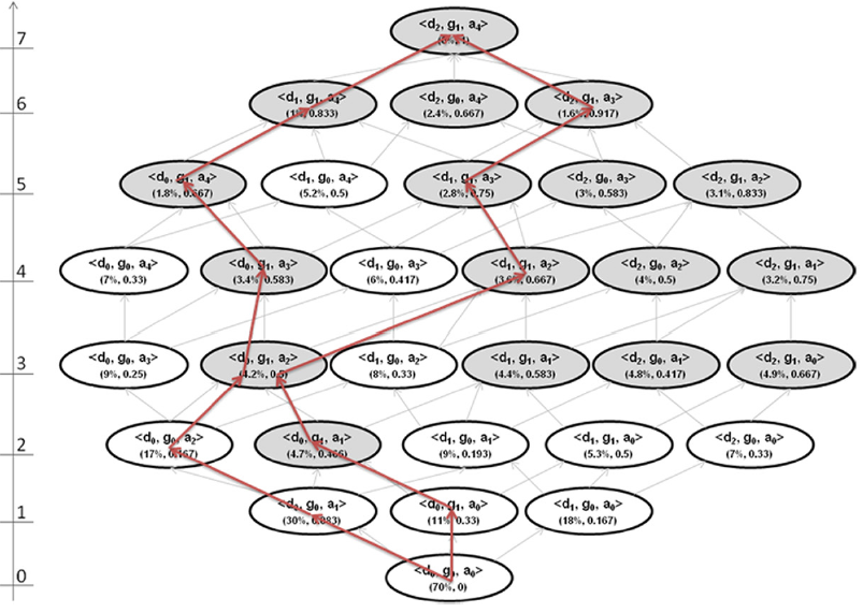
\includegraphics[width=1.0\textwidth]{lattice.png}
	\caption{Generalization Lattice\cite{el2009globally}}%
	\label{lattice}
\end{figure}


\begin{algorithm}[H]
\caption{The OLA Algorithm works in 3 Steps:}
\While{not all generalization strategies are compared}
{
For every generalization strategy I build a binary search to find all k-anonymous nodes K in I\\
For every I that includes k-anonymous nodes save the one with the least Information loss L in I\\
Compare I to respect of the information loss\\
The one with the lowest Information loss of all L is the global optimum solution\\
\Return{global optimal solution}
}
\end{algorithm}

The information loss can be measured with three possible matrices. The height of each generalized attribute can be taken as a measure. An example can be found in figure  \ref{Generalization}, because if we generalize on the Level d1, then we would have an information loss of one. The problem with this kind of measurement is that it does not take into account the height of the whole generalization tree. If we would generalize the gender of a person then we would have only one possibility, i.e. the specific gender or no information at all. With the first measurement, one would also be able to measure an information loss of one. In order to eliminate this problem, the Prec measurement can be used. This measurement takes into account the total possible height of the generalization tree. It can be measured with the formula:\\\\ \ $\frac{Number of levels generalized}{Number of possible generalization levels} = Information Loss$\\\\The last possibility is of measuring information loss in the OLA algorithm with the Discernability Metric(DM). This gives a penalty to each record which is indistinguishable from other records. As such, the less one generalizes, the less penalties will occur. Another barrier to the general practice of k-anonymity algorithm is that it measures the information loss in its data set. After all, the anonymized dataset will be used in datamining applications and there is no possibility to measure the information loss regarding the goal of the data mining target. It is possible to discover an optimal k-anonymity solution with the OLA algorithm but due to the fact it is an NP-hard problem there is also a possibilty not to find a solution.\cite{el2009globally}.



\subsection{Cloaking Algorithm}
Moving object data creates new challenges to a traditional database, data mining, and privacy-preserving technologies due to its unique characteristics. It is time-dependent, location-dependent, and is generated in large volumes of high-dimensional stream data. The following algorithm provides an example of privacy production. The Cloaking Algorithm tries to produce anonymity on location-based data for users of Location Bases Services(LBS). The Cloaking Algorithm is installed on a location protection broker on a trusted server and anonymize messages which will afterward send to the LBS. K-anonymity prevents such a privacy breach by ensuring that each individual record can only be released if there is at least k-1 other (distinct) individuals whose associated records are indistinguishable from the former in terms of their quasi-identifier values. There a two possible attacks which can obtain  the identity of a sender of a message. In  Restricted Space Identification, the attacker (A) observes that message (M) is sent from location(L). He then detects the background knowledge that L belongs to someone specific. For example, if Mr. Bob the owner of a flat sends a message and the attacker observes this message. He can re-link the identity of Bob. Another attack is  Observation Identification. If A has observed the current location L of subject S and finds a message M from L then A learns that S has sent M. To prevent this leaking of information the cloaking algorithm works with Spatial Cloaking and Temporal Cloaking. Spatial Cloakings goal is to increase the location from where M is sended in such a way that there are more messages in this area. So that there is not only one message at a time in one area. Temporal Cloaking extends the sending time until more messages are in one area. With both of these technics the algorithm tries to produce k-anonymity for m different messages. Temporal Cloaking enables the possibility of delaying a message until enough messages are in one location, but this will harm the usability of the LBSs. In their paper Gedik and Liu show that it is possible to implement the algorithm on a real world example, but it will lack the utility of the LBS because of the delayed messages \cite{gedik2004customizable}.



\section{High-Dimensional Transaction Data}

Transaction data is typically high-dimensional. Shopping sites like Amazon.com include millions of catalog items, which could all be a potential QID. Therefore, this type of data must include k-anonymities before being published\cite{wang2010privacy}. Aggarwal in his paper "On k-Anonymity and the Curse of Dimensionality", reports that this task is impossible to achieve. In his example, they work with a clustering K-anonymity algorithm like The KACA Algorithm and try to archive 2-anonymity on a $3*10^8$ dimensional dataset. He argues that by having an increase in the dimension of the dataset and by aiming to achieve k-anonymity, the information loss will increase rapidly up to a point that it is impractical for specific applications ( e.g. data mining tools).  The reason for that is the curse of high dimensionality which does not allow the clustering of points in high dimensional space, because of the great space between them. Xu introduced a method to get at least a bit of practical usage. He claimed that an attack knows at least n-different transactions of a victim and concludes that some information cannot be accessed because that would is effort consumin\cite{xu2008publishing}. Thus, the background knowledge of an attacker can be bounded. In practice, to anonymize high dimensional datasets can be a problematic \cite{aggarwal2005k}.

%\section{Releated techniques}

\section{Summary}
<<<<<<< HEAD
The distortion of the data-section attests the great importance of algorithms as  the one shown in KACA-Algorithm (Section 4.1), which address the problem of data distortion. This algorithm no only enables the production of tables which include more information, but also retains their k-anonymity. As it was shown in the OLA algorithm sub-section, there are various possibilities of choosing between different information loss metrics which all compute different values to the same k-anonymous node. Therefore, it is the implementer’s task to choose which one suits the best to his data. Different metrics have different advantages and disadvantages, which have to be compared. Although the implementer can measure the information loss on his dataset, a comparison of the information loss to the upcoming data mining tool or machine learning application would be more interesting. The information loss metrics themselves do not reveal which information are important for the upcoming data mining step. \\\\
=======
The distortion of the data-section attests the great importance of algorithms as  the one shown in KACA-Algorithm (Section 4.1), which address the problem of data distortion. This algorithm no only enables the production of tables which include more information, but also retains their k-anonymity.  Data distortion is just a synonym for information loss and both got the same definition.
As it was shown in at OLA algorithm (Section 4.2), there are various possibilities of choosing between different information loss metrics which all compute different values to the same k-anonymous node. Therefore, it is the implementer’s task to choose which one suits the best to his data. Different metrics have different advantages and disadvantages, which have to be compared\cite{el2009globally}. Although the implementer can measure the information loss on his dataset, a comparison of the information loss to the upcoming data mining tool or machine learning application would be more interesting. The information loss metrics themselves do not reveal which information are important for the upcoming data mining step. \\\\
>>>>>>> d2a0079e29e39f9c5de8ff63792a3ab1c121259f

Additionally, suppression can also harm the quality of the data, thus it should be chosen wisely. The production of k-anonymity is linked to a NP-Hard problem which results in a difficult implementation in real-time applications as shown by the Cloaking Algorithm (Section 4.3). This complexity can result in problems in finding an optimal solution in real-world data sets and can make a practical implementation difficult \cite{meyerson2004complexity}. High Dimensional Data like transaction data with more than thousands of attributes are in practice not capable to produce k-anonymity for all attributes. The reason for this, is the so-called Curse of High Dimensionality(Section 5) which produces a metric space that is very large for producing k-anonymity solutions for all attributes \cite{aggarwal2005k}. A possible solution is provided by the so-called bounded background knowledge, in which some attributes cannot be used as a quasi-identifier, since the effort of obtaining the background knowledge linked to the attributes is estimated too high. \\\\

As shown in the Attacks chapter(Section 3.2), attacks can be considered as barriers against k-anonymity. They are not only a threat to the anonymity of the user, but they can also result in identity disclosure. The cloaking algorithm provides a good example of the connection between anonymity and usability. The anonymization of the data reduces the usability of location-based services. This is the case due to the construction of the Spatial cloaking and Temporal cloaking boxes, because they have to contain enough messages to constrain them and let the become k-anonymous. The Software provides the option that a user of the client can decide how much usability he wants to sacrifice in the sake of anonymity. As a result, the user can control how much utility he wants to give up \cite{gedik2004customizable}. The implementation of K-anonymity results in different kind of problems we shown that NP-Hard, information loss, attacks against k-anonymity and utility loss can be barriers for a implementation.

\newpage
\bibliography{literature}
\bibliographystyle{splncs03}

\end{document}


